\documentclass[border=10pt]{standalone}
\usepackage{tikz}
\usepackage{amsmath}
\usetikzlibrary{arrows.meta, positioning, fit, backgrounds, calc}

\begin{document}
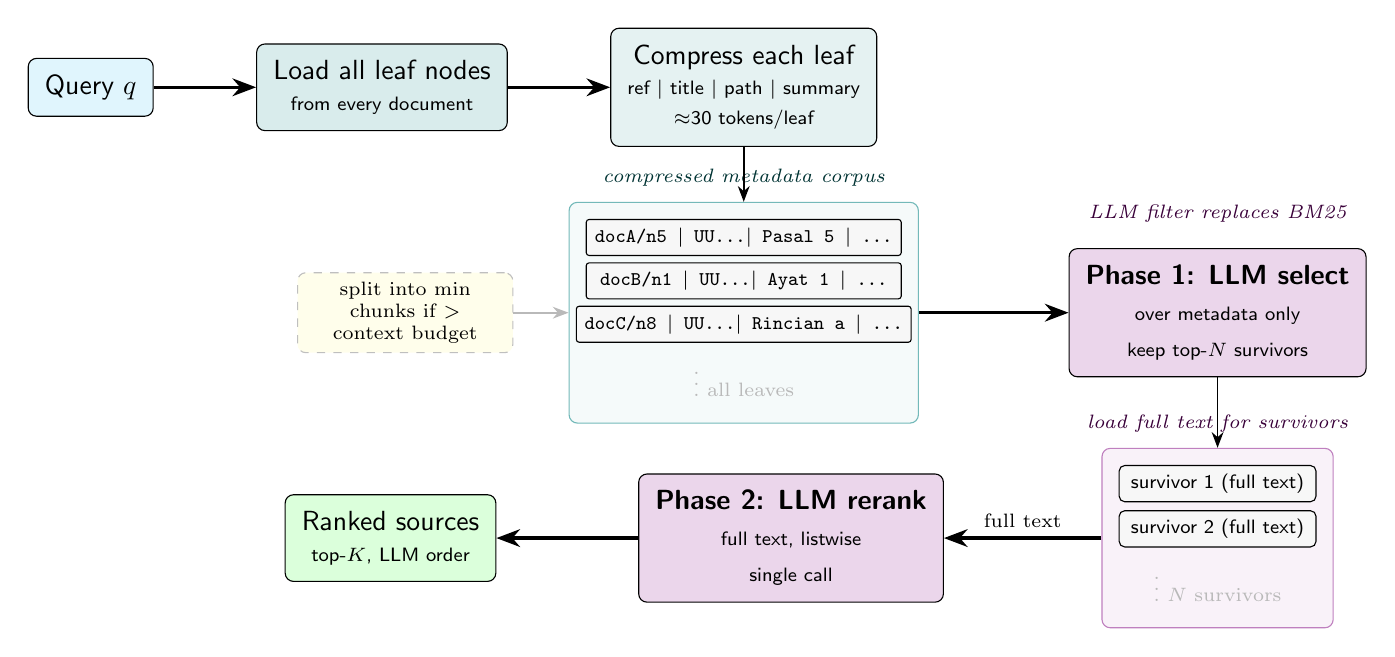
\begin{tikzpicture}[
    font=\small,
    box/.style={draw, rounded corners=3pt, align=center, font=\sffamily,
                inner sep=6pt},
    line/.style={draw, rounded corners=1pt, minimum width=4.0cm, minimum height=0.4cm,
                 font=\scriptsize\ttfamily, align=left, inner sep=3pt, fill=gray!6},
    cand/.style={draw, rounded corners=2pt, minimum width=2.5cm, minimum height=0.46cm,
                 font=\scriptsize\sffamily, align=left, inner sep=3pt, fill=gray!6},
    flow/.style={-{Stealth[length=3mm]}, very thick},
    arr/.style={-{Stealth[length=2mm]}, semithick},
]

    %==================== QUERY ====================
    \node[box, fill=cyan!12] (q) {Query $q$};

    %==================== LOAD ALL LEAVES ====================
    \node[box, fill=teal!15, right=1.3cm of q, align=center] (load)
        {Load all leaf nodes\\[-1pt]{\scriptsize from every document}};
    \draw[flow] (q) -- (load);

    %==================== COMPRESS step ====================
    \node[box, fill=teal!10, right=1.3cm of load, align=center] (compress)
        {Compress each leaf\\[-1pt]{\scriptsize ref $|$ title $|$ path $|$ summary}\\[-1pt]
         {\scriptsize $\approx$30 tokens/leaf}};
    \draw[flow] (load) -- (compress);

    %==================== compressed metadata list ====================
    \node[line] (m1) at ($(compress.south)+(0,-1.15)$) {docA/n5 $|$ UU\ldots $|$ Pasal 5 $|$ \ldots};
    \node[line, below=0.08cm of m1] (m2) {docB/n1 $|$ UU\ldots $|$ Ayat 1 $|$ \ldots};
    \node[line, below=0.08cm of m2] (m3) {docC/n8 $|$ UU\ldots $|$ Rincian a $|$ \ldots};
    \node[font=\scriptsize, text=gray!55, below=0.04cm of m3] (mdots) {$\vdots$ all leaves};

    \begin{scope}[on background layer]
        \node[draw=teal!55, rounded corners=3pt, fill=teal!4,
              fit=(m1)(mdots), inner sep=6pt] (metabox) {};
    \end{scope}
    \node[font=\scriptsize\itshape, text=teal!40!black, anchor=south]
        at ([yshift=2pt]metabox.north) {compressed metadata corpus};
    \draw[arr] (compress.south) -- (metabox.north);

    %==================== chunk note ====================
    \node[draw=gray!50, dashed, rounded corners=3pt, fill=yellow!8, font=\scriptsize,
          align=center, left=0.7cm of metabox, text width=2.5cm] (chunk)
        {split into min chunks if $>$ context budget};
    \draw[arr, gray!55] (chunk.east) -- (metabox.west);

    %==================== PHASE 1: LLM metadata select ====================
    \node[box, fill=violet!16, right=1.9cm of metabox, align=center, minimum height=1.5cm]
        (phase1) {\textbf{Phase 1: LLM select}\\[1pt]{\scriptsize over metadata only}\\[1pt]
                  {\scriptsize keep top-$N$ survivors}};
    \draw[flow] (metabox.east) -- (phase1.west);

    %==================== survivors pool ====================
    \node[cand] (s1) at ($(phase1.south)+(0,-1.35)$) {survivor 1 (full text)};
    \node[cand, below=0.1cm of s1] (s2) {survivor 2 (full text)};
    \node[font=\scriptsize, text=gray!55, below=0.04cm of s2] (sdots) {$\vdots$ $N$ survivors};

    \begin{scope}[on background layer]
        \node[draw=violet!50, rounded corners=3pt, fill=violet!5,
              fit=(s1)(sdots), inner sep=6pt] (survbox) {};
    \end{scope}
    \node[font=\scriptsize\itshape, text=violet!45!black, anchor=south]
        at ([yshift=2pt]survbox.north) {load full text for survivors};
    \draw[arr] (phase1.south) -- (survbox.north);

    %==================== PHASE 2: LLM full-text rerank ====================
    \node[box, fill=violet!16, left=2.0cm of survbox, align=center, minimum height=1.5cm]
        (phase2) {\textbf{Phase 2: LLM rerank}\\[1pt]{\scriptsize full text, listwise}\\[1pt]
                  {\scriptsize single call}};
    \draw[flow] (survbox.west) -- node[above, font=\scriptsize] {full text} (phase2.east);

    %==================== OUTPUT ====================
    \node[box, fill=green!14, left=1.8cm of phase2, align=center] (out)
        {Ranked sources\\[-1pt]{\scriptsize top-$K$, LLM order}};
    \draw[flow] (phase2.west) -- (out.east);

    %==================== filter contrast note ====================
    \node[font=\scriptsize\itshape, text=violet!45!black, above=0.2cm of phase1]
        {LLM filter replaces BM25};

\end{tikzpicture}
\end{document}